\section{INFORMACIÓN GENERAL} 

\begin{itemize}
\subsection{Objetivos:}

	 \item Aprender y utilizar una importante herramienta como Azure Data Studio para la Monitorización de Base de Datos mediante Auditoría.
\subsection{Requerimientos}


	
    Para el desarrollo de esta práctica se requerirá de los siguientes        	  conocimientos básicos:
	\item Conocimientos básicos de administración de base de datos 	  			 Microsoft SQL Server.
	\item Conocimientos básicos de SQL.\\\\
	
	\item Tener Azure Data Studio Instalado.\\
	
	\begin{figure}[htb]
	\begin{center}
	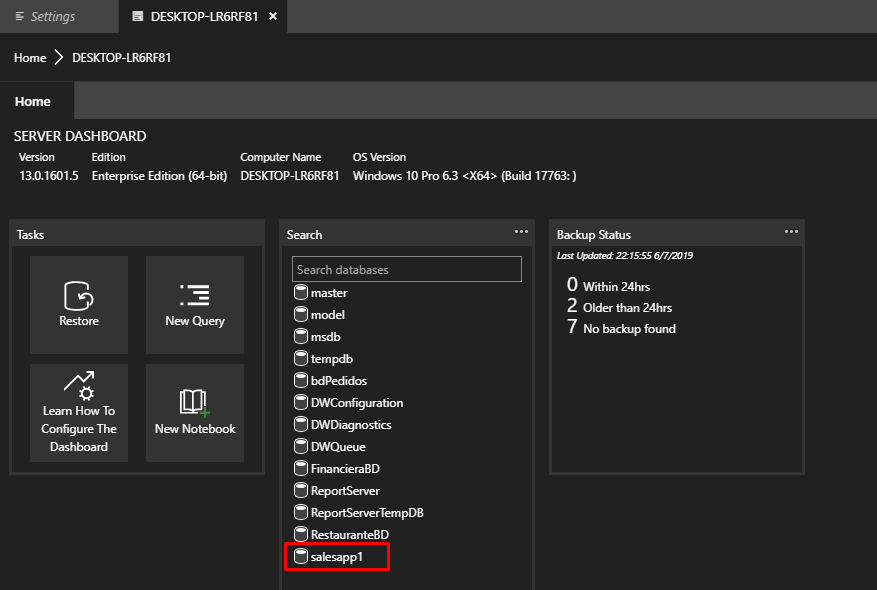
\includegraphics[width=15cm]{./Imagenes/audit0}
	\end{center}
	\end{figure}


\end{itemize}